We are now ready to present experimental results of \sys performance. We start with describing the hardware environment (Section~\ref{sec:results_hardware}) followed by the software environment (Section~\ref{sec:results_software}) and we concluded by the evaluation results (Section~\ref{sec:results_evaluation}).

\subsection{Hardware Suite Description}
\label{sec:results_hardware}

In the experiments we used WISP\,5.1~\cite{wisp5,wisp} (with MSP430FR5969~\cite{wolverine} 64\,kB FRAM) or MSP430XXX launchpad~\cite{} (hardware type will be specified per experiment in Section~\ref{sec:results_evaluation}). WISP\,5.1 has been programmed using TI FET for experiments. FET was also used as a power supply in non-intermittent power experiment. To measure energy consumption of the applications (refer to Section~\ref{sec:results_software}) EDB~\cite{edb} was used. In experiments involving wireless power, WISP was powered through RFID reader (Impinj R1000 with firmware version 3.2.4.240~\cite{r1000_data_sheet}) connected to Liard RFMAX S9028PCRJ 8\,dBic~\cite{atlas2015}. RFID reader is controlled by a PC running Ubuntu 10.4 executing open source Python-based \emph{sllurp} library~\cite{sllrp_github} enabling low-level RFID reader control. Transmitted power of the RFID reader was 30\,dBm at 915\,MHz center frequency. For distance controlled experiments, WISP was positioned at hollow paper tubes placed directly on a lying antenna. 

\subsection{Software Suite Description}
\label{sec:results_software}

We compare \sys against state of the art intermittent execution approach---Chain~\cite{chain}. We need to note that although another very relevant task-based runtime has been recently presented and referenced many times throughout this paper---Alpaca~\cite{alpaca}---we did not have the access to its code during the preparation of this manuscript. 

The applications that were used in the evaluation are given in Table~\ref{table:benchmark_list}. These benchmarks are the same ones as used in~\cite{chain,alpaca}.

\begin{table}
	\begin{tabular}{|c|c|c|}
		\hline
		Name & SLOC (\sys) & SLOC (Chain~\cite{chain})\\
		\hline\hline
		Temperature sensing & 388 & 721 \\ %53\%
		Cuckoo & 483 & 762 \\ %63\%
		RSA & 887 & 1233 \\ %71\%
		DFT & --- & --- \\ %Two resolutions: 4 and 8 Bytes
		Huffman & --- & --- \\ %Data decompression size: 100 bytes
		Selection sort & --- & --- \\
		\hline
	\end{tabular}
\caption{List of benchmark programs used in \sys evaluation; SLOC: source lines of code.}
\label{table:benchmark_list}
\end{table}

\subsection{Evaluation}
\label{sec:results_evaluation}

\subsubsection{Compiler Performance}
\label{sec:results_compiler}

Compiler experiment: taskifying completion time of a code run, correctness (manual inspection---proof by example), comparison manual/automatic taskification - fixed power supply

\todo{Provide structure to this section}{Kiwan}

\subsubsection{}
\label{sec:}

\begin{figure}
	\centering
	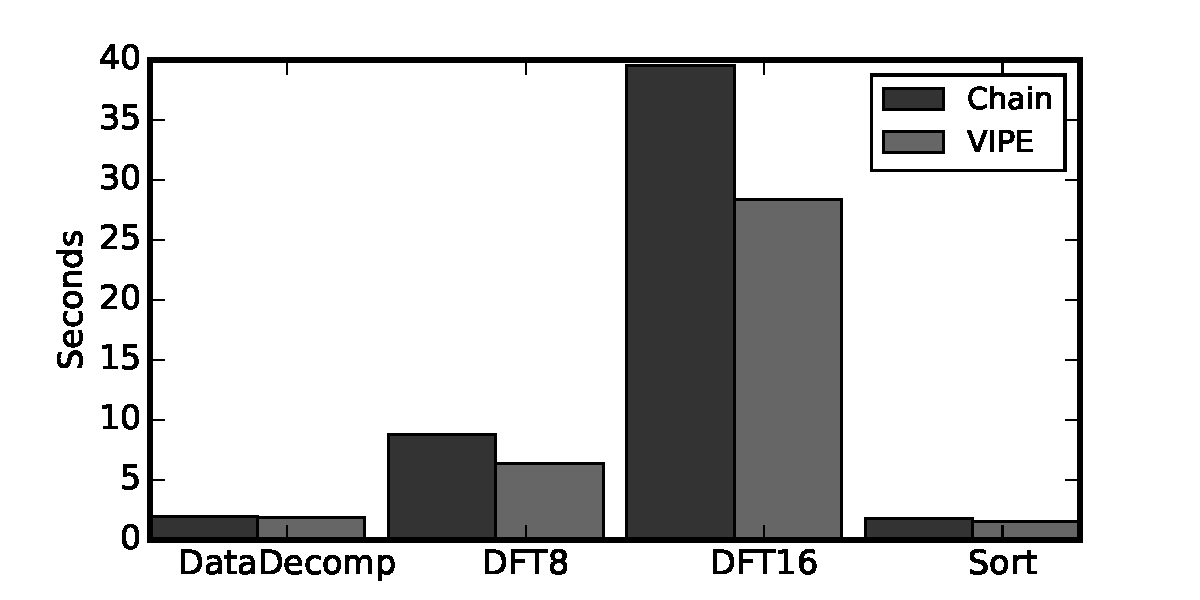
\includegraphics[width=\columnwidth]{figures/chain_vipe}
	\caption{Time to complete for a set of testing applications (refer to Table~\cite{table:benchmark_list}) using \sys versus Chain.}
	\label{fig:IPOSPerformance}
\end{figure}

Fig.~\ref{fig:IPOSPerformance} shows that \sys requires a shorter execution time to execute an application under the modular execution model. The size of the virtual task that \sys uses is one real task, i.e. no task coalescing is applied.

Task coalescing experiment: with WISP at 3 distances and with fixed power, for all apps, compared against chain, show amount of task merged, time to completion, overhead (in terms of what?), energy consumed with fixed power

\subsubsection{Memory Management}
\label{sec:results_memory_management}

Paging/memory experiment: page swapping cost (execution time)---comparing against chain and full double buffering approach, show number of page swaps, 

\todo{Provide argument for page swapping using hardware support}{Brandon}

\subsubsection{Case Study}
\label{sec:case_study}

Battery-less microphone: with \sys and without \sys, compared against Chain.